\section{Supervisión de servidor de archivos (FTP/FTP Server File Count)}
\subsection{Sensor FTP}
\subsection{Instalación}
Para la utilización de este sensor, se realizó primero la instalación del servidor FTP en una máquina virtual Ubuntu Server, en la cual se ingresó el comando \textbf{sudo apt-get install vsftpd}, mostrado en la figura \ref{image:ftp1} mismo que instalaba las librerías necesarias de este servidor.

\FloatBarrier
\begin{figure}[htbp!]
		\centering
			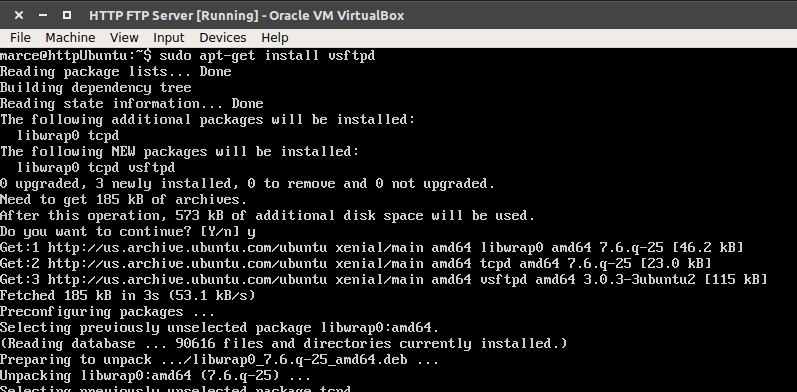
\includegraphics[width=.9 \textwidth]{images/ftp1}
		\caption{Comando de instalación FTP.}
		\label{image:ftp1}
\end{figure}
\FloatBarrier

Posteriormente, ya que se había realizado toda la descarga de paquetes, se ingreso mediante el comando \textbf{sudo nano /etc/vsftpd.conf}, como lo muestra la figura \ref{image:ftp2} con el fin de eliminar el comentario de la línea \textbf{write\_enable = YES} y de esta manera permitir la escritura de archivos dentro del servidor.

\FloatBarrier
\begin{figure}[htbp!]
		\centering
			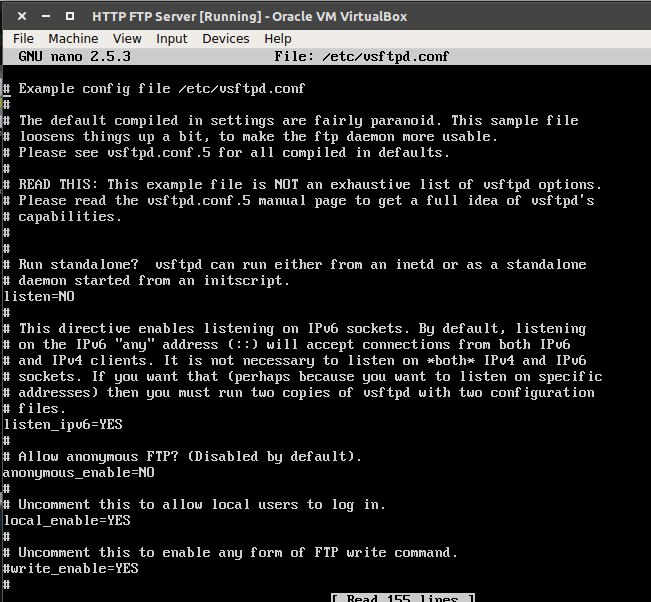
\includegraphics[width=.75 \textwidth]{images/ftp2}
		\caption{Archivo de configuración FTP.}
		\label{image:ftp2}
\end{figure}
\FloatBarrier

Por último, se ejecutó el comando \textbf{sudo service vsftp restart} con el cual se reinicia el servicio FTP y posteriormente el comando \textbf{sudo service vsftp status} para asegurarnos de que el estado del servicio sea activo. Por último únicamente se obtuvo la ip de la máquina virtual para saber el host al cual se enviarían y se recibirían los datos almacenados en dicho servidor (figura \ref{image:ftp3}).

\FloatBarrier
\begin{figure}[htbp!]
		\centering
			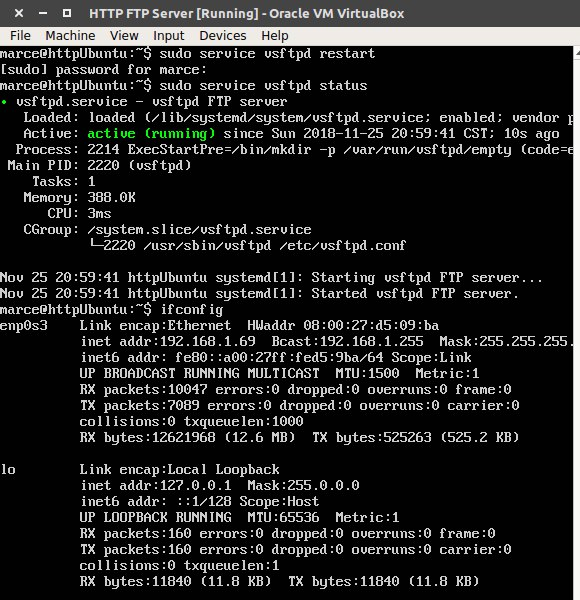
\includegraphics[width=.75 \textwidth]{images/ftp3}
		\caption{Reinicio de servicio y status FTP.}
		\label{image:ftp3}
\end{figure}
\FloatBarrier
\subsection{Funcionamiento}
En cuanto al funcionamiento de este sensor, se tenían dos diferentes opciones que se desplegaban en el menú al ejecutar el programa cliente.py, dichas opciones eran tanto importar como exportar un archivo al servidor FTP (figura \ref{image:ftp4}).

\FloatBarrier
\begin{figure}[htbp!]
		\centering
			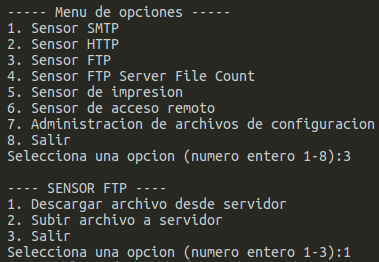
\includegraphics[width=.6 \textwidth]{images/ftp4}
		\caption{Opciones de sensor FTP.}
		\label{image:ftp4}
\end{figure}
\FloatBarrier
Ya que se seleccionó en este caso la opción 1, se solicitan ciertos datos para poder acceder al servidor y obtener la información de este (figura \ref{image:ftp6}).
\FloatBarrier
\begin{figure}[htbp!]
		\centering
			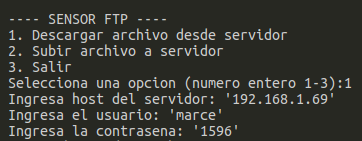
\includegraphics[width=.6 \textwidth]{images/ftp6}
		\caption{Archivos disponibles en servidor FTP.}
		\label{image:ftp6}
\end{figure}
\FloatBarrier
Una vez que se ingresó al servidor, se despliegan todos los archivos disponibles en una carpeta en particular y se solicita al usuario el archivo que desea importar desde el servidor y por último se muestra toda la información perteneciente al archivo descargado como el nombre, los bytes y el tiempo que se tardó en transmitirse dicho archivo (figura \ref{image:ftp7}).
\FloatBarrier
\begin{figure}[htbp!]
		\centering
			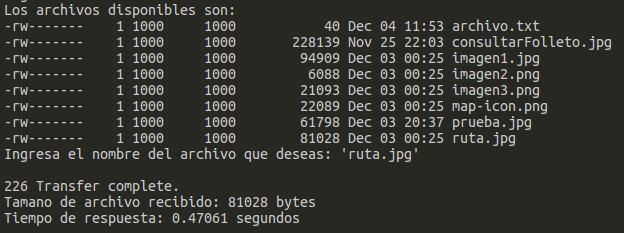
\includegraphics[width=.75 \textwidth]{images/ftp7}
		\caption{Solicitud de descarga de archivo vía FTP.}
		\label{image:ftp7}
\end{figure}
\FloatBarrier

Por otro lado, en caso de que se presione la opción 2 para subir un archivo al servidor, se muestra únicamente el tiempo de ejecución y de igual manera la respuesta del servidor y la información del archivo transmitido (figura \ref{image:ftp8}).

\FloatBarrier
\begin{figure}[htbp!]
		\centering
			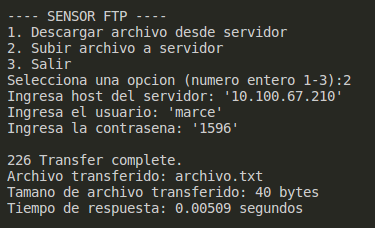
\includegraphics[width=.6 \textwidth]{images/ftp8}
		\caption{Información del archivo enviado al servidor FTP.}
		\label{image:ftp8}
\end{figure}
\FloatBarrier

Si verificamos en el servidor, se observa que el archivo fue transmitidos correctamente y cuando se abre el archivo enviado, se visualizan los nombres de los alumnos integrantes del equipo (figuras \ref{image:ftp9} y \ref{image:ftp10}).

\FloatBarrier
\begin{figure}[htbp!]
		\centering
			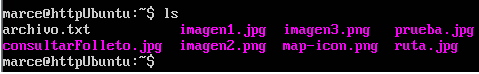
\includegraphics[width=.75 \textwidth]{images/ftp9}
		\caption{Archivos dentro del servidor FTP.}
		\label{image:ftp9}
\end{figure}
\FloatBarrier

\FloatBarrier
\begin{figure}[htbp!]
		\centering
			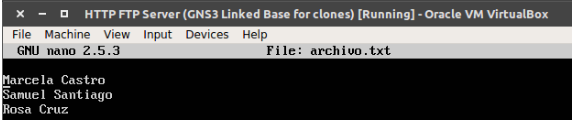
\includegraphics[width=.75 \textwidth]{images/ftp10}
		\caption{Contenido del archivo enviado al servidor FTP.}
		\label{image:ftp10}
\end{figure}
\FloatBarrier
Por último se muestra e código de ejecución tanto para obtener un archivo desde el servidor, como para subir un nuevo archivo a este (figuras \ref{image:ftpc1} y \ref{image:ftpc2}). 
\FloatBarrier
\begin{figure}[htbp!]
		\centering
			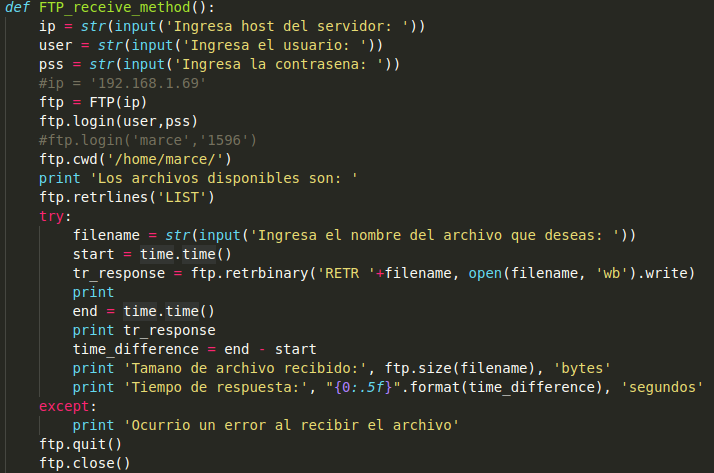
\includegraphics[width=.75 \textwidth]{images/ftpc1}
		\caption{Código para descargar un archivo del servidor FTP.}
		\label{image:ftpc1}
\end{figure}
\FloatBarrier
\FloatBarrier
\begin{figure}[htbp!]
		\centering
			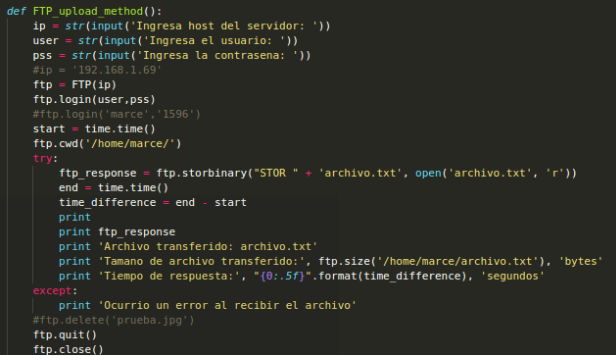
\includegraphics[width=.8 \textwidth]{images/ftpc2}
		\caption{Código para subir un archivo del servidor FTP.}
		\label{image:ftpc2}
\end{figure}
\FloatBarrier
\subsection{Sensor FTP Server File Count}
\subsection{Instalación}
Para la implementación del contador de archivos que almacena el servidor FTP se realiza una conexión SSH y se enlistan y se cuentan los archivos en el directorio de almacenamiento del servidor. Para ello se utiliza el siguiente comando:\\
\texttt{ls -1 /home/ftp/ | wc -l}\\

El código se puede observar en la figura \ref{image:ftpcounter}.

\FloatBarrier
\begin{figure}[htbp!]
		\centering
			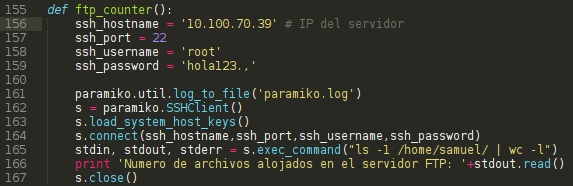
\includegraphics[width=.75 \textwidth]{images/ftpcounter}
		\caption{Código del contador de archivos en el servidor FTP.}
		\label{image:ftpcounter}
\end{figure}
\FloatBarrier
\subsection{Funcionamiento}
El funcionamiento se puede ver en la figura \ref{image:ftpcounterfunc}.

\FloatBarrier
\begin{figure}[htbp!]
		\centering
			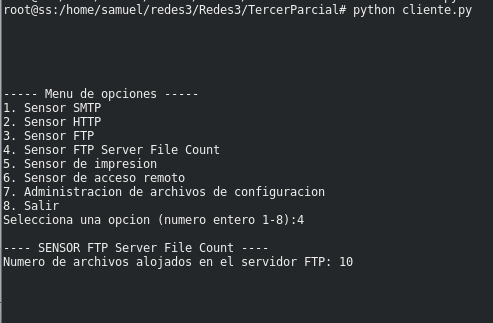
\includegraphics[width=.75 \textwidth]{images/ftpcounterfunc}
		\caption{Contador de archivos en el servidor FTP.}
		\label{image:ftpcounterfunc}
\end{figure}
\FloatBarrier